\documentclass{ximera}

\input{../../../preamble.tex}


\definecolor{fvdnavy}{HTML}{071D43}
\definecolor{fvdcyan}{HTML}{20BFC6}
\definecolor{fvdcyanlight}{HTML}{EFFCFB}
\definecolor{fvdmagenta}{HTML}{F10D69}
\definecolor{fvdmagentalight}{HTML}{FFF1F7}
\definecolor{fvdtext}{HTML}{163044}





%=================================================
% Pedagogische omgevingen
% PDF: tcolorbox
% HTML: learning-box
%=================================================

\newenvironment{voorkennis}
{%
    \ifdefined\HCode
        \HCode{%
<section class="learning-box learning-box--prior">
<div class="learning-box__header">
<span class="learning-box__icon" aria-hidden="true"></span>
<span class="learning-box__title">Voorkennis</span>
</div>
<div class="learning-box__content">
        }%
        \begin{itemize}
    \else
       \begin{tcolorbox}[
    enhanced,
    breakable,
    colback=fvdcyanlight,
    colframe=fvdcyan,
    coltext=fvdtext,
    boxrule=0.5pt,
    leftrule=4pt,
    arc=4mm,
    outer arc=4mm,
    left=7mm,
    right=6mm,
    top=5mm,
    bottom=5mm,
    before skip=6mm,
    after skip=6mm,
    title=Voorkennis,
    coltitle=fvdcyan,
    fonttitle=\bfseries\Large,
    attach title to upper={\par\smallskip},
    boxed title style={
        empty,
        left=0mm,
        right=0mm,
        top=0mm,
        bottom=0mm
    },
    overlay={
        \draw[
            fvdcyan,
            line width=0.5pt
        ]
        ([xshift=42mm,yshift=-13mm]frame.north west)
        --
        ([xshift=-7mm,yshift=-13mm]frame.north east);
    }
]
        \begin{itemize}
    \fi
}
{%
    \end{itemize}
    \ifdefined\HCode
        \HCode{%
</div>
</section>
        }%
    \else
        \end{tcolorbox}
    \fi
}


\newenvironment{leerdoelen}
{%
    \ifdefined\HCode
        \HCode{%
<section class="learning-box learning-box--goals">
<div class="learning-box__header">
<span class="learning-box__icon" aria-hidden="true"></span>
<span class="learning-box__title">Leerdoelen</span>
</div>
<div class="learning-box__content">
        }%
        \begin{itemize}
    \else
\begin{tcolorbox}[
    enhanced,
    breakable,
    colback=fvdmagentalight,
    colframe=fvdmagenta,
    coltext=fvdtext,
    boxrule=0.5pt,
    leftrule=4pt,
    arc=4mm,
    outer arc=4mm,
    left=7mm,
    right=6mm,
    top=5mm,
    bottom=5mm,
    before skip=6mm,
    after skip=6mm,
    title=Leerdoelen,
    coltitle=fvdmagenta,
    fonttitle=\bfseries\Large,
    attach title to upper={\par\smallskip},
    boxed title style={
        empty,
        left=0mm,
        right=0mm,
        top=0mm,
        bottom=0mm
    },
    overlay={
        \draw[
            fvdmagenta,
            line width=0.5pt
        ]
        ([xshift=42mm,yshift=-13mm]frame.north west)
        --
        ([xshift=-7mm,yshift=-13mm]frame.north east);
    }
]
        \begin{itemize}
    \fi
}
{%
    \end{itemize}
    \ifdefined\HCode
        \HCode{%
</div>
</section>
        }%
    \else
        \end{tcolorbox}
    \fi
}



\title{Hoe verandert een functie?}
\author{Ingmar Herreman}

\begin{document}

% FVD_CHAPTER_DATA_START
% Automatisch gegenereerd uit index.tex.
% Niet handmatig aanpassen.
\fvdchapterdata{5}{Het gedrag van functies beschrijven}{3}
% FVD_CHAPTER_DATA_END




\fvdchapterdata{5}{Het gedrag van functies beschrijven}{3}

\begin{abstract}
Twee functies kunnen allebei stijgen en toch heel verschillend veranderen.
In dit hoofdstuk verfijnen we daarom onze beschrijving: stijgt of daalt een functie
aan een constant tempo, steeds sneller of steeds trager?
\end{abstract}

\maketitle

\begin{voorkennis}

    \item Je kunt uit een grafiek aflezen waar een functie stijgt, daalt of constant is.
  
    \item Je kunt lokale maxima en minima herkennen in een grafiek.
  
    \item Je kunt functiewaarden bepalen en verschillen tussen functiewaarden met elkaar vergelijken.
  
    \item Je kunt informatie uit grafieken en tabellen aflezen en interpreteren.
  
  \end{voorkennis}
  
  \begin{leerdoelen}
  
    \item Je kunt het onderscheid uitleggen tussen stijgen of dalen enerzijds en de manier waarop die stijging of daling zelf verandert anderzijds.
  
    \item Je kunt constante, toenemende en afnemende stijging herkennen in een grafiek en het verschil tussen deze vormen van stijging beschrijven.
  
    \item Je kunt constante, toenemende en afnemende daling herkennen in een grafiek en het verschil tussen deze vormen van daling beschrijven.
  
    \item Je kunt de verandering van een functie onderzoeken door veranderingen van functiewaarden bij gelijke stappen van de invoer met elkaar te vergelijken.
  
    \item Je kunt uit een tabel, grafiek of concrete context afleiden en beschrijven hoe de stijging of daling van een functie evolueert.
  
    \item Je kunt op basis van gegeven informatie over stijgen, dalen en de verandering daarvan een mogelijke grafiek schetsen.
  
    \item Je kunt uitspraken over de manier waarop een functie verandert kritisch onderzoeken en je conclusie wiskundig motiveren.
  
    \item Je kunt de manier waarop een functie verandert interpreteren binnen een betekenisvolle STEM-context en je conclusie terugkoppelen naar de oorspronkelijke situatie.
  
  \end{leerdoelen}


% ============================================================
% 1. STIJGEN IS NIET ALTIJD HETZELFDE STIJGEN
% ============================================================

\FVDsection{Stijgen is niet altijd hetzelfde stijgen}

In het vorige hoofdstuk beschreven we \emph{of} een functie stijgt of daalt.
Maar daarmee is nog niet alles gezegd.

Vergelijk bijvoorbeeld drie situaties:

\begin{itemize}
  \item een auto waarvan de afgelegde afstand elke seconde met \(20\) m toeneemt;
  \item een vallend voorwerp dat per seconde steeds meer afstand aflegt;
  \item een opwarmend voorwerp waarvan de temperatuur nog stijgt, maar steeds trager.
\end{itemize}

In alle drie kan de onderzochte grootheid stijgen.
Toch gebeurt dat niet op dezelfde manier.

We stellen daarom een verfijnde vraag:

\[
\important{
\text{Hoe verandert de verandering zelf wanneer }x\text{ toeneemt?}
}
\]

\begin{center}
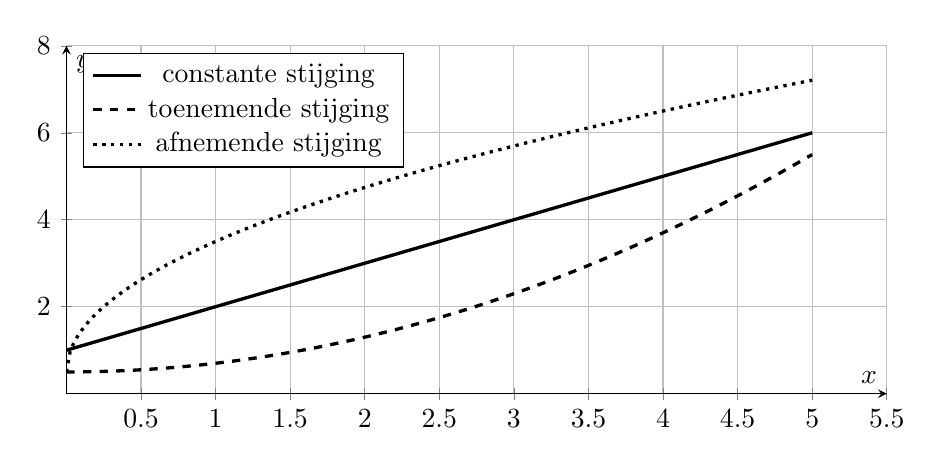
\begin{tikzpicture}
\begin{axis}[
 width=12cm,height=6cm,
 axis lines=middle,
 xmin=0,xmax=5.5,ymin=0,ymax=8,
 xlabel={$x$},ylabel={$y$},
 grid=both,samples=200,
 legend style={at={(0.02,0.98)},anchor=north west}
]
\addplot[very thick,domain=0:5] {1+x};
\addlegendentry{constante stijging}
\addplot[very thick,dashed,domain=0:5] {0.2*x^2+0.5};
\addlegendentry{toenemende stijging}
\addplot[very thick,dotted,domain=0:5] {3*sqrt(x)+0.5};
\addlegendentry{afnemende stijging}
\end{axis}
\end{tikzpicture}
\end{center}

Alle drie de grafieken stijgen. Het verschil zit in de manier waarop hun helling evolueert.


% ============================================================
% 2. KIJK NAAR GELIJKE STAPPEN
% ============================================================

\FVDsection{Vergelijk gelijke stappen}

Een eerste manier om verandering te onderzoeken is functiewaarden vergelijken
bij \textbf{gelijke stappen in \(x\)}.

Beschouw de tabel:

\[
\begin{array}{c|ccccc}
x&0&1&2&3&4\\
\hline
f(x)&1&2&4&7&11
\end{array}
\]

De toename bij elke stap van \(1\) in \(x\) is:

\[
+1,\qquad +2,\qquad +3,\qquad +4.
\]

De functie stijgt dus niet alleen: de stijging wordt steeds groter.

\begin{definitie}
Als bij gelijke toenames van \(x\) de toename van \(f(x)\)
steeds groter wordt, spreken we van \textbf{toenemende stijging}.

Als die toename steeds kleiner wordt maar positief blijft,
spreken we van \textbf{afnemende stijging}.

Als de toename telkens dezelfde is, spreken we van
\textbf{constante stijging}.
\end{definitie}

\begin{opmerking}
We vergelijken veranderingen alleen eerlijk wanneer de stappen in de invoer gelijk zijn.
Een toename over \(1\) seconde rechtstreeks vergelijken met een toename over \(5\) seconden
kan misleidend zijn.
\end{opmerking}


% ============================================================
% 3. DRIE MANIEREN VAN STIJGEN
% ============================================================

\FVDsection{Constante, toenemende en afnemende stijging}

\begin{eigenschap}[Constante stijging]
Bij constante stijging neemt \(f(x)\) bij gelijke stappen in \(x\)
telkens met hetzelfde bedrag toe. De grafiek heeft een constante helling.

Een rechte met positieve richtingscoëfficiënt is het typische voorbeeld.
\end{eigenschap}

\begin{eigenschap}[Toenemende stijging]
Bij toenemende stijging wordt de grafiek van links naar rechts steeds steiler omhoog.
Bij gelijke stappen in \(x\) worden de positieve veranderingen in \(f(x)\) groter.
\end{eigenschap}

\begin{eigenschap}[Afnemende stijging]
Bij afnemende stijging stijgt de functie nog steeds, maar steeds trager.
De grafiek wordt van links naar rechts minder steil.
Bij gelijke stappen in \(x\) worden de positieve veranderingen in \(f(x)\) kleiner.
\end{eigenschap}

\begin{voorbeeld}[Drie tabellen]

\[
\begin{array}{c|ccccc}
x&0&1&2&3&4\\ \hline
f(x)&1&3&5&7&9
\end{array}
\]
heeft veranderingen \(+2,+2,+2,+2\): constante stijging.

\[
\begin{array}{c|ccccc}
x&0&1&2&3&4\\ \hline
g(x)&0&1&4&9&16
\end{array}
\]
heeft veranderingen \(+1,+3,+5,+7\): toenemende stijging.

\[
\begin{array}{c|ccccc}
x&0&1&2&3&4\\ \hline
h(x)&0&4&7&9&10
\end{array}
\]
heeft veranderingen \(+4,+3,+2,+1\): afnemende stijging.
\end{voorbeeld}


% ============================================================
% 4. DALEN KAN OOK OP VERSCHILLENDE MANIEREN
% ============================================================

\FVDsection{Constante, toenemende en afnemende daling}

Ook een dalende functie kan op verschillende manieren dalen.

\begin{definitie}
Bij \textbf{constante daling} neemt \(f(x)\) bij gelijke stappen in \(x\)
telkens met hetzelfde bedrag af.

Bij \textbf{toenemende daling} wordt de afname steeds sterker:
de grafiek daalt steeds steiler.

Bij \textbf{afnemende daling} blijft de functie dalen,
maar wordt de afname steeds kleiner:
de grafiek vlakt af.
\end{definitie}

\begin{center}
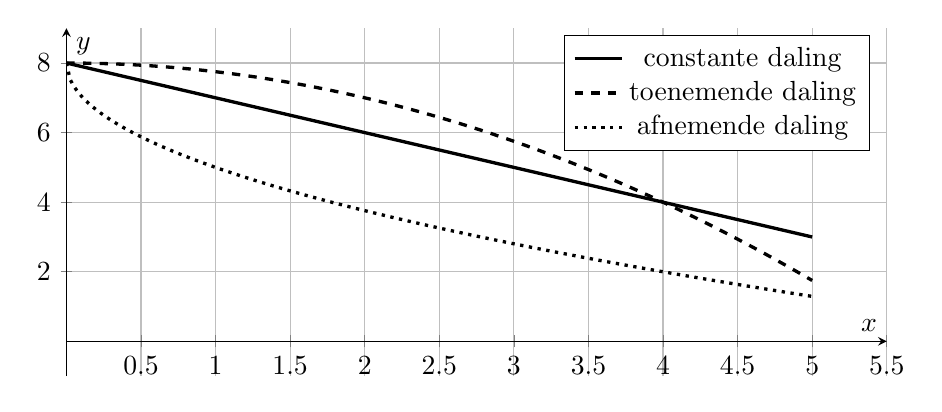
\begin{tikzpicture}
\begin{axis}[
 width=12cm,height=6cm,
 axis lines=middle,
 xmin=0,xmax=5.5,ymin=-1,ymax=9,
 xlabel={$x$},ylabel={$y$},
 grid=both,samples=200,
 legend style={at={(0.98,0.98)},anchor=north east}
]
\addplot[very thick,domain=0:5] {8-x};
\addlegendentry{constante daling}
\addplot[very thick,dashed,domain=0:5] {8-0.25*x^2};
\addlegendentry{toenemende daling}
\addplot[very thick,dotted,domain=0:5] {8-3*sqrt(x)};
\addlegendentry{afnemende daling}
\end{axis}
\end{tikzpicture}
\end{center}

\begin{opmerking}[Let op de taal]
``Toenemende daling'' betekent niet dat de functiewaarden toenemen.
De functie \emph{daalt}; de sterkte van die daling neemt toe.

``Afnemende daling'' betekent evenmin dat de functie stijgt.
Ze daalt nog steeds, maar steeds minder sterk.
\end{opmerking}


% ============================================================
% 5. EEN OVERZICHT
% ============================================================

\FVDsection{Twee vragen, zes situaties}

Bij het analyseren van een grafiek stellen we voortaan twee vragen:

\[
\boxed{
\begin{array}{c}
\text{1. Stijgt of daalt de functie?}\\[1mm]
\text{2. Wordt die stijging of daling sterker, zwakker of blijft ze constant?}
\end{array}}
\]

Dat geeft:

\[
\begin{array}{c|c|c}
\text{verloop} & \text{verandering} & \text{grafische indruk}\\
\hline
\text{stijgend} & \text{constant} & \text{even steil omhoog}\\
\text{stijgend} & \text{toenemend} & \text{steeds steiler omhoog}\\
\text{stijgend} & \text{afnemend} & \text{steeds vlakker omhoog}\\
\text{dalend} & \text{constant} & \text{even steil omlaag}\\
\text{dalend} & \text{toenemend} & \text{steeds steiler omlaag}\\
\text{dalend} & \text{afnemend} & \text{steeds vlakker omlaag}
\end{array}
\]


% ============================================================
% 6. HELLING ZONDER AFGELEIDEN
% ============================================================

\FVDsection{Kijken naar helling — nog zonder afgeleiden}

We gebruiken hier het woord \textbf{helling} kwalitatief:
we vergelijken hoe steil een grafiek is.

\begin{itemize}
  \item positieve helling \(\Rightarrow\) de functie stijgt;
  \item negatieve helling \(\Rightarrow\) de functie daalt;
  \item een steeds grotere positieve helling \(\Rightarrow\) toenemende stijging;
  \item een positieve helling die kleiner wordt \(\Rightarrow\) afnemende stijging;
  \item een steeds sterker negatieve helling \(\Rightarrow\) toenemende daling;
  \item een negatieve helling die naar \(0\) evolueert \(\Rightarrow\) afnemende daling.
\end{itemize}

\begin{opmerking}[Vooruitblik]
Later krijgt dit idee een exacte wiskundige taal via afgeleiden.
Dan zullen we de helling zelf als functie onderzoeken.
Hier bouwen we eerst het grafische inzicht op dat daarvoor nodig is.
\end{opmerking}


% ============================================================
% 7. VERANDERINGSPUNTEN
% ============================================================

\FVDsection{Waar verandert het soort verandering?}

Een grafiek kan bijvoorbeeld eerst toenemend stijgen en daarna afnemend stijgen.

\begin{center}
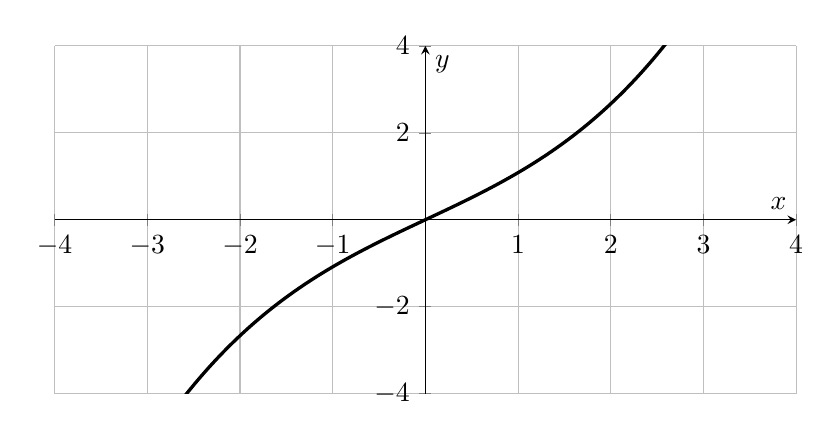
\begin{tikzpicture}
\begin{axis}[
 width=11cm,height=6cm,
 axis lines=middle,
 xmin=-4,xmax=4,ymin=-4,ymax=4,
 xlabel={$x$},ylabel={$y$},
 grid=both,samples=200
]
\addplot[very thick,domain=-3.5:3.5] {x^3/12+x};
\end{axis}
\end{tikzpicture}
\end{center}

De manier waarop de helling evolueert kan dus veranderen zonder dat de functie
ophoudt met stijgen.

We beschrijven in dit hoofdstuk vooral \emph{wat} we grafisch waarnemen.
De formele studie van kromming, buigpunten en tweede afgeleiden komt later,
wanneer de nodige analysetechnieken beschikbaar zijn.

\begin{opmerking}
Een verandering van toenemende naar afnemende stijging is niet automatisch
een maximum. Bij een maximum verandert het verloop van stijgend naar dalend.
Hier kan de functie aan beide kanten blijven stijgen.
\end{opmerking}


% ============================================================
% 8. STEM-CONTEXT: BEWEGING
% ============================================================

\FVDsection{STEM-context: beweging}

Stel dat \(s(t)\) de afgelegde afstand van een voertuig voorstelt.

Als de afstand in opeenvolgende seconden toeneemt met

\[
5,\ 5,\ 5,\ 5\ \text{m},
\]

dan neemt de afstand constant toe.

Als de toenames zijn

\[
2,\ 4,\ 6,\ 8\ \text{m},
\]

dan legt het voertuig per seconde steeds meer afstand af:
de stijging van \(s\) neemt toe.

Als de toenames zijn

\[
8,\ 6,\ 4,\ 2\ \text{m},
\]

dan neemt de afstand nog steeds toe, maar steeds minder snel:
de stijging van \(s\) neemt af.

\begin{opmerking}[Interpretatie]
Bij een afstand-tijdgrafiek zegt de steilheid iets over hoe snel de afstand verandert.
Zo vormt deze grafische analyse een natuurlijke brug tussen wiskunde en beweging in de fysica.
\end{opmerking}


% ============================================================
% 9. STEM-CONTEXT: OPWARMEN
% ============================================================

\FVDsection{STEM-context: opwarming}

Een voorwerp wordt in een warme omgeving geplaatst.
De temperatuur \(T(t)\) stijgt, maar het temperatuurverschil met de omgeving
wordt steeds kleiner.

Typisch zien we dan:

\[
\text{stijgend}
\qquad+\qquad
\text{steeds minder steil}.
\]

We spreken van \textbf{afnemende stijging}.

\begin{center}
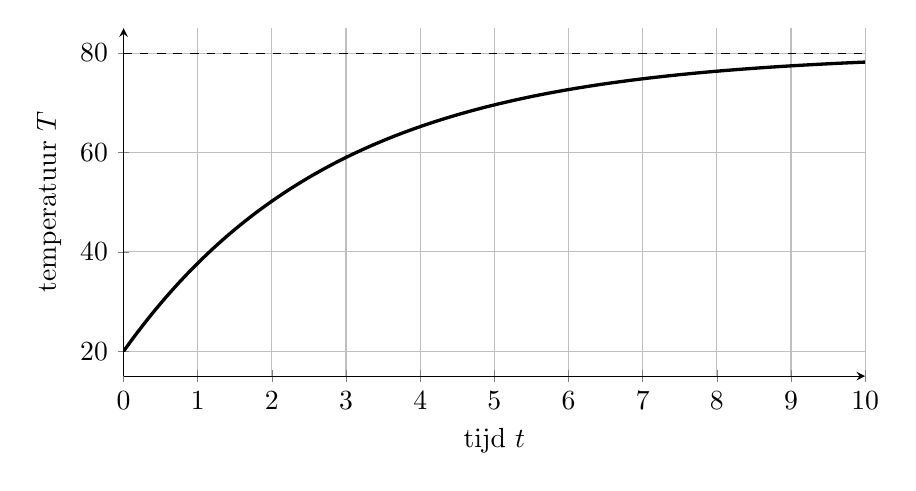
\begin{tikzpicture}
\begin{axis}[
 width=11cm,height=6cm,
 axis lines=left,
 xmin=0,xmax=10,ymin=15,ymax=85,
 xlabel={tijd \(t\)},ylabel={temperatuur \(T\)},
 grid=both,samples=200
]
\addplot[very thick,domain=0:10] {80-60*exp(-0.35*x)};
\addplot[dashed,domain=0:10] {80};
\end{axis}
\end{tikzpicture}
\end{center}

De temperatuur blijft toenemen, maar de grafiek vlakt af naarmate ze
de omgevingstemperatuur nadert.


% ============================================================
% 10. GEOGEBRA
% ============================================================

\FVDsection{Onderzoeken met GeoGebra}

Onderzoek in GeoGebra de functies

\[
f(x)=x,\qquad
g(x)=x^2,\qquad
h(x)=\sqrt{x}
\]

op \(x\geq 0\).

\begin{enumerate}
  \item Alle drie stijgen. Beschrijf waarin hun stijging verschilt.
  \item Kies \(x=0,1,2,3,4\) en vergelijk de opeenvolgende functiewaarden.
  \item Welke grafiek heeft constante stijging?
  \item Welke heeft toenemende stijging?
  \item Welke heeft afnemende stijging?
  \item Leg uit hoe de tabel en de grafiek dezelfde conclusie ondersteunen.
\end{enumerate}

Onderzoek daarna

\[
p(x)=-x,\qquad
q(x)=-x^2,\qquad
r(x)=-\sqrt{x}
\]

op \(x\geq0\) en formuleer de overeenkomstige uitspraken over daling.

\begin{opmerking}
Gebruik GeoGebra om te onderzoeken en te controleren.
De uiteindelijke conclusie moet je zelf in wiskundige taal kunnen formuleren en motiveren.
\end{opmerking}


% ============================================================
% 11. SAMENVATTING
% ============================================================

\FVDsection{Samenvatting}

\[
\important{
\text{stijgen of dalen}
\longrightarrow
\text{helling vergelijken}
\longrightarrow
\text{constant, toenemend of afnemend veranderen}
}
\]

Onthoud:
\begin{itemize}
  \item stijgen/dalen en toenemende/afnemende stijging/daling zijn verschillende kenmerken;
  \item vergelijk bij tabellen veranderingen over gelijke stappen in \(x\);
  \item toenemende stijging betekent steeds steiler omhoog;
  \item afnemende stijging betekent stijgen maar afvlakken;
  \item toenemende daling betekent steeds steiler omlaag;
  \item afnemende daling betekent dalen maar afvlakken;
  \item constante stijging of daling hoort bij een constante helling;
  \item de formele studie met afgeleiden volgt later.
\end{itemize}

\end{document}
